%%%%%%%%%%%%%%%%%%%%%%%%%%%%%%%
% CHAPTER 4: EXPLORATORY STUDY
% 	RESULTS 1 - COMPARISON
% File: tex/expstudy-chapter/expstudy-results1-comparison.tex
%%%%%%%%%%%%%%%%%%%%%%%%%%%%%%%%%%%%%%%%%%%%%%%%
%%%%%%%%%%%%%%%%%%%%%%%%%%%%%%%%%%%%%%%%%%%%%%%%
\newpage
\section{Results: Comparing PIM Behaviour}
\label{exp-study:Results-comparison}
%%%%%%%%%%%%%%%%%%%%%%%%%%%%%%%%%%%%%%%%%%%%%%%%
%%%%%%%%%%%%%%%%%%%%%%%%%%%%%%%%%%%%%%%%%%%%%%%%
%During analysis of the data a number of patterns and common themes began to emerge despite the wide range of strategies, concerns, and dispositions regarding PIM practice.  
%The following sections attempt to highlight general tendencies from the data that held across the majority of users. However at the same time important exceptions are highlighted.
%Due to the wide variance in user behaviour, it is emphasised that the results are suggestive/indicative only.

%%%%%%%%%%%%%%%%%%%%%%%%%%%%%%%%%%%%%%%%%%%%%%%%%%%%%%%%%%%%
% TO ADD: WHY WAS THIS DONE? WHAT IS THE MAIN CONCLUSION?
%%%%%%%%%%%%%%%%%%%%%%%%%%%%%%%%%%%%%%%%%%%%%%%%%%%%%%%%%%%%

%%%%%%%%%%%%%%%%%%%%%%%%%%%%%%%%%%%
% Summary and structure overview
%%%%%%%%%%%%%%%%%%%%%%%%%%%%%%%%%%%
% State: generalized/aggregate across all participants
% Relate to method? Content analysis in Section X
% The nature of Barreau's sub-activities (acquisition, organization, maintenance and retrieval)~\citep{barreau:95} between the file, email and bookmark collections.
% The bulk of the section is structured in terms of the conceptual framework outlined in \textbf{Chapter~\ref{chapter:bg}}.
% \textbf{Sections~\ref{exp-study:comparison-acquisition}}, \textbf{~\ref{exp-study:comparison-organization}}, \textbf{~\ref{exp-study:comparison-maintenance}}, and \textbf{~\ref{exp-study:comparison-retrieval}} deal with the .  
% PIM BEHAVIOUR COMPARISON
% \textbf{Section~\ref{exp-study:behaviour-comparison}} discusses the high-level comparison of PIM behaviour between the 3 tools in terms of the four sub-activities outlined in \textbf{Chapter~\ref{chapter:bg}}: acquisition, organization, maintenance, and retrieval.
The next four sections compare typical PIM behaviour between files, email and bookmarks in terms of the 4 PIM sub-activities outlined in \textbf{Chapter~\ref{chapter:bg}}: acquisition, organization, maintenance, and retrieval. Finally, \textbf{Section~\ref{exp-study:Results-comparison-summary}} summarises the key observations.

%%%%%%%%%%%%%%%%%%%%%%%%%%%%%%%%%%%%%%%%%%%%%%%%
\subsection{Acquisition and Collection Characteristics}
\label{exp-study:comparison-acquisition}
%%%%%%%%%%%%%%%%%%%%%%%%%%%%%%%%%%%%%%%%%%%%%%%%

Barreau defined acquisition as \textit{``the methods and rules by which information becomes part of the PIM system''}~\citep{barreau:95}. \textbf{Table~\ref{table:chapter3_acquisition_strategy}} compares the main characteristics of acquisition behaviour between the PIM tools.

%%%%%%%%%%%%%%%%%%%%%%%%%%%%%%%%%%%%%%%%%%%%%%%%%%%%%%%%%%
% TABLE: Comparing acquisition practices regarding file, email and bookmarks}
%%%%%%%%%%%%%%%%%%%%%%%%%%%%%%%%%%%%%%%%%%%%%%%%%%%%%%%%%%
\begin{table}[hbtp]
\begin{center}
\begin{footnotesize}
\setlength{\extrarowheight}{2pt}
\begin{tabular}{|p{2.5cm}|p{3.5cm}|p{3.5cm}|p{3.5cm}|}
% Table generated by Excel2LaTeX from sheet 'ACQUISITION'
\hline
    {\bf } & {\bf Document File} & {\bf Email} & {\bf Web Bookmark} \\
\hline
{\bf Item acquisition} & Manual creation. User decides what to add. & Automatic creation on download. User decides what to keep. & Manual creation. User decides what to add. \\
\hline
{\bf Creation rate of items} & Low. Most common participant estimate: 1-5 per day. & High (up to many 100s per day) & Low. Most common participant estimate: 1-5 per week. \\
\hline
{\bf Naming of items} & Each file must have a unique name. & Default "name" is defined by subject as specified by sender. Hard to change. & Default name is title of the page to which bookmark refers. \\
\hline
{\bf Standard implicit metadata } & Date created, date modified, size, author. & Date received, from, to, message thread, size. & Date created, date modified, size, author. \\
\hline
{\bf Problems reported} & Naming of files. & Ascertaining value of new email. Changing message subject. & Default name often unsatisfactory and hard to change. \\
\hline
\end{tabular}    
\end{footnotesize}
\caption{Comparison of acquisition behaviour between files, email and bookmarks}
\label{table:chapter3_acquisition_strategy}
\end{center}
\end{table}


% In our study WE noted substantial differences regarding the acquisition of document files and web bookmarks on one hand, and email on the other.
% The acquisition of document files and web bookmarks is under the user's explicit control. Items are added to the collection manually as driven by their needs and interests. In contrast email acquisition is effectively uncontrolled.
% Any items sent to the user concerned appears in their collection be it important work mail or distracting spam.
Two very different modes of acquisition were observed. In the document file and web bookmark collections, acquisition is \textit{explicit}: the user decides what items to add. In email, acquisition is \textit{implicit}.  The onus is on the user to assess the value of items and decide what to delete, P11: \textit{``everything just gets stuffed into the inbox -- basically the whole world has write access''}.   % Participant descriptions highlighted how the \textit{nature of acquisition} varies between the tools - from manual in files and bookmarks, to uncontrolled in email.  
Several participants had developed elaborate schemes for managing newly arrived messages, e.g. P21: \textit{``I try to keep it [the inbox] as small as possible, so it acts as a to-do list. I have another folder called `Diverse' which is stuff to deal with that's been tidied from inbox''}.  A number of participants also used filters to organize mailing list messages and delete spam.
% The user has little control over what items are added beyond specifying when new messages are downloaded, using mail filters to delete spam, and unsubscribing from mailing lists.  

% For some users the presence of unwanted messages was not a problem. Others noted the significant amount of effort involved in processing new email:

\textbf{Table~\ref{table:chapter3_item_characteristics}} compares the underlying characteristics of the items stored in each collection, and the nature of each collection as a whole. 
% This section also summarises the general characteristics of the collections of document files, email and web bookmarks. 
% These characteristics are referred to later in the chapter as factors contributing to the choice of particular PIM strategies (\textit{CHECK}).
Emails are clearly differentiated in terms of \textit{authorship} -- the majority of email messages are authored by users other than the owner of the email collection.
For this reason there is a need for users to ascertain the value of email messages after they have been acquired.  In contrast, files and web bookmarks are created by the owner of the collection.  
A second key difference is in terms of item \textit{form}. Email messages and most files contain some form of information, much of which has been authored or edited by the managing user. In contrast, web bookmarks are \textit{references} to content stored remotely on websites \footnote{Document file collections also facilitate the creation of references that point to other files. These are known as \textit{short-cuts} under MS Windows or \textit{links} under UNIX. However in this study only one participant mentioned the regular use of links within their file collection (in their case a link to a network drive from their UNIX home directory). File links were observed more frequently for managing applications on the desktop.}.

% As noted above all participants actively collected both files and email. 
The three collections also differed in terms of their \textit{value} to their owner.  File collections were highly prized, and many participants expressed the pride they felt towards the contents, much of which they had kept over a number of years, P9: \textit{``Some of them I'll need again, some of the things I'm quite proud of ... why should I throw it away? It doesn't cost me anything''}. Email collections were valued less than files, but most participants noted the sentimental or professional value of a subset of their messages, \textit{P24: ``I keep them to make sure I've got one thing from them to reply to. Also it's nice that the person has written''}. Bookmarks were of low importance for most participants, supporting findings in~\citep{kftf:01}. However, all but one collected them to some extent. Bookmarks were valued less due to: (1) the existence of other ways of re-accessing websites, e.g. search engines, and (2) websites' ephemeral nature, P1: \textit{``It's often not worth the overhead of adding links, I only use the pages once or twice. And then there's the overhead of managing the organization''}.  Bookmark collections were very small (tens of items), compared to file and email (thousands of items). 


%%%%%%%%%%%%%%%%%%%%%%%%%%%%%%%%%%%%%%%%%%%%%%%%%%%%%%%%%%
% TABLE: Comparing characteristics of file, email and bookmarks}
%%%%%%%%%%%%%%%%%%%%%%%%%%%%%%%%%%%%%%%%%%%%%%%%%%%%%%%%%%
\begin{table}[hbtp]
\begin{center}
\begin{footnotesize}
\setlength{\extrarowheight}{2pt}
\begin{tabular}{|p{2.5cm}|p{3.5cm}|p{3.5cm}|p{3.5cm}|}
% Table generated by Excel2LaTeX from sheet 'CHARACTERISTICS'
\hline
{\bf Characteristics} & {\bf Document File} & {\bf Email} & {\bf Web Bookmark} \\
\hline
{\bf Management interface} & Graphical file manager, icons on desktop, command-line. & Email application. & Web browser application. \\
\hline
{\bf Size of collection} & Large (many hundreds). & Very large (thousands). & Small (tens). \\
\hline
{\bf Authorship of item content} & Many files authored by owner.  Some authored by other users (e.g. downloads).  & Majority of emails authored by other users. Some may be self-addressed or copies of sent messages. & Bookmarks do not contain content. \\
\hline
{\bf Form of items} & Most contain content (e.g. text).  May contain embedded bookmarks or files. Also, possible to create links (short-cuts).  & Contain content. May contain "attached" files or bookmarks. & References to remote web pages on the internet. \\
\hline
{\bf Homogeneity of items} & Many different technological formats for files (e.g. text, image). & Common technological format & Common technological format \\
\hline
{\bf Age of collection} & Many years. Many files are kept over the long-term (e.g. over job changes) & A few years. Relatively more ephemeral then files (e.g. collection  restarted after job-change). & Most bookmarks tend to be ephemeral. Collection often abandoned and restarted. \\
\hline
{\bf Importance/value of collection} & Very important. Many files are highly valued. & Subset of messages highly-valued (typically recent messages in inbox).  & Only small subset valued. \\
\hline
{\bf Context of collection} & Personal document file collection co-exists with system files in file system. & Stand-alone collection, although stored on file system. & Stand-alone collection, although stored on file system. \\
\hline
\end{tabular}  
\end{footnotesize}
\caption{Comparing the characteristics of files, email and web bookmarks}
\label{table:chapter3_item_characteristics}
\end{center}
\end{table}
\normalsize


%%%%%%%%%%%%%%%%%%%%%%%%%%
% \subsubsection{Summary}
%%%%%%%%%%%%%%%%%%%%%%%%%%
%%%%%%%%%%%%%%%%%%%%%%%%%%%%%%%%%%%%%%%%%%%%%%%%%%%%%%%%%%%%
% TO ADD: WHY WAS THIS DONE? WHAT IS THE MAIN CONCLUSION?
%%%%%%%%%%%%%%%%%%%%%%%%%%%%%%%%%%%%%%%%%%%%%%%%%%%%%%%%%%%%
% \textit{TODO: summarize key findings from the acquisition section. The next section moves on to comparing organization practices between the three tools.}





%%%%%%%%%%%%%%%%%%%%%%%%%%%%%%%%%%%%%%%%%%%%%%%%
\subsection{Organization}
\label{exp-study:comparison-organization}
%%%%%%%%%%%%%%%%%%%%%%%%%%%%%%%%%%%%%%%%%%%%%%%%
%	IN DISCUSSION: Carefully differentiate organization (incremental ongoing filing/tidying) and maintenance (occasional spring-cleaning).
%	ADD/DEVELOP STATS: median, p-values for comparison?}
%	ADD: hierarchy fan-out (interpret as use of small/large categories?
%%%%%%%%%%%%%%%%%%%%%%%%%%%%%%%%%%%%%%%%%%%%%%%%%%%%%%%%%%%%
% \textit{TODO. Highlight key findings: variety, classification. \textbf{Figure~\ref{fig:chapter1_collection_forms}} illustrates the typical forms of the document file, email and web bookmark collections that WE encountered.}  
% %%%%%%%%%%%%%%%%%%%%%%%%%%%%%
% FIGURE - FOLDER SHAPES
%\begin{figure}[hbtp]
%	\begin{center}
%		\leavevmode
%		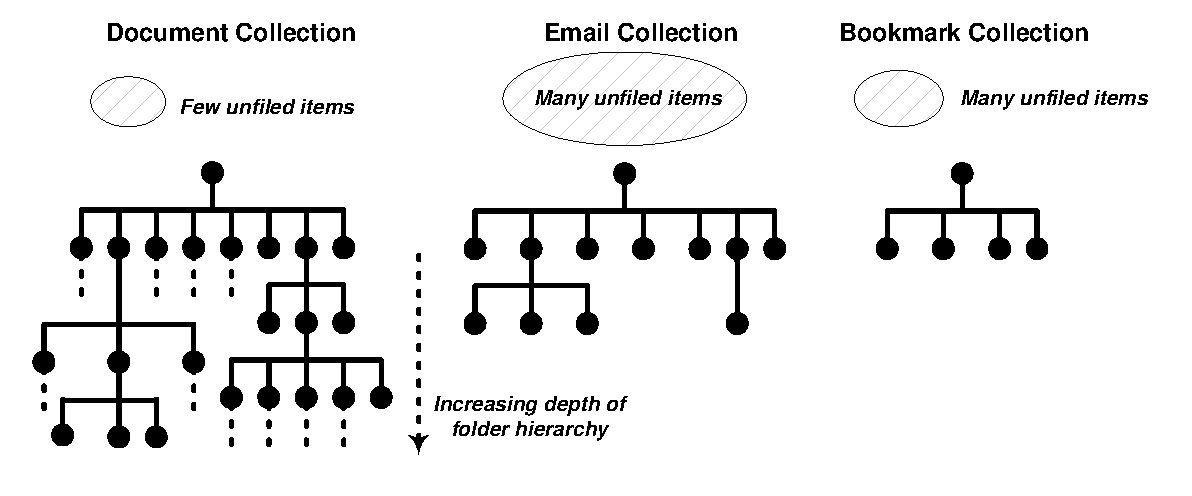
\includegraphics[width= \textwidth]{pictures/exp-study/exp-study-OrgComparison.pdf}
%		\caption{Comparison of the typical form of folder hierarchies developed in each PIM collection}
%		\label{fig:chapter1_collection_forms}
%	\end{center}
%\end{figure}
%%%%%%%%%%%%%%%%%%%%%%%%%%%%%%%%%%%%%%%%%%%%%%%%%%%%%%%%%%%%
% In the conceptual overview of PIM presented in \textbf{Chapter~\ref{chapter:introduction}}, two forms of organization were considered: (1) \textit{implicit} organization based on system-assigned metadata, (2) \textit{explicit} organization performed by the user (e.g. classifying items within folders or spatially grouping items on the desktop).
% The study focused on participants' explicit folder-based organizing behaviour, rather than reliance on implicit metadata or the use of the desktop to spatially organize items.
% Overall the document file collection tended to be structured much more extensively with the vast majority of items filed within folders for most users. 
% On average the file folder hierarchies were almost twice as deep as the email and web bookmark hierarchies (see \textbf{Table~\ref{table:chapter3_organization_strategy}}). 
\textbf{Table~\ref{table:chapter3_organization_strategy}} shows an overview comparison of organizing behaviour across the 3 PIM-tools. This analysis is based on the qualitative data and initial analysis of the folder structures.

%%%%%%%%%%%%%%%%%%%%%%%%%%%%%%%%%%%%%%%%%%%%%%%%%%%%%%%%%%
% TABLE: Comparing organizing characteristics of file, email and bookmarks}
%%%%%%%%%%%%%%%%%%%%%%%%%%%%%%%%%%%%%%%%%%%%%%%%%%%%%%%%%%
% CONSIDER ADDING: Consider use of large/small categories, default folders
% Barreau: different classifying rules based upon level of granularity to support in workload
\begin{table}[hbtp]
\begin{center}
\begin{footnotesize}
\setlength{\extrarowheight}{2pt}
\begin{tabular}{|p{2.5cm}|p{3.5cm}|p{3.5cm}|p{3.5cm}|}
% Table generated by Excel2LaTeX from sheet 'ORGANIZATION'
\hline
    {\bf } & {\bf Document File} & {\bf Email} & {\bf Web Bookmark} \\
\hline
{\bf Participants with active folders} &   {\it 25} &   {\it 23} &   {\it 16} \\
\hline
{\bf Average number of folders} & {\it 49 (SD: 30, min: 5, max: 122)} & {\it 37 (SD: 41, min: 0, max: 181)} & {\it 12 (SD: 15, min: 0, max: 55)} \\
\hline
{\bf Average maximum depth of folders} & {\it 3.0 (SD: 1.6, min: 1, max: 7)} & {\it 1.7 (SD: 1.2, min: 0, max: 4)} & {\it 1.1 (SD: 0.9, min: 0, max: 3)} \\
\hline
{\bf Average number of unfiled items} & {\it 65 (SD: 104, min: 0, max: 340)} & {\it 777 (SD: 1235, min: 7, max: 5577)} & {\it 43 (SD: 47, min: 0, max: 200)} \\
\hline
{\bf Most common organizing behaviour} & "One touch" file-on-creation. Occasional spring-cleaning..  & Some incremental filing but many left in inbox.  Use of filters to file mailing lists. Occasional spring-cleaning..  & Mostly left in default chronological order. Occasional spring-cleaning. Folder structures often abandoned. \\
\hline
{\bf Extent of filing} & High: most files organized in folders. & Variable. Large number of unfiled items in "inbox". & Majority in chronologically ordered list. \\
\hline
{\bf Location of "active" items} & Most active files located in folders. Some participants had unfiled "work-in-progress" area. & Inbox. Occasional project folders. & Most likely to be recently added unfiled items. \\
\hline
{\bf Other  organizing mechanisms (non-folder based) } & Spatial placement on desktop. Use of different  drives and partitions. & Occasional separation of roles between different email accounts. & Occasional spatial placement on desktop. Use of ``links bar''. \\
\hline
{\bf Key  problems} & Anxiety of order. Keeping collection tidy (unfiled items, pruning folders).  & Anxiety of order (focused on size of inbox). & Anxiety of order. Time to organize outweighs value of doing so (items rarely used again). Poor interface. \\
\hline
\end{tabular}  
\end{footnotesize}
\caption{Comparing organizing behaviour between files, email and bookmarks}
\label{table:chapter3_organization_strategy}
\end{center}
\end{table}

% Also consider use of command-line
% Note that other collections of personal information such as contacts and to-do items were rarely organized explicitly.
% Since organizing strategies varied significantly between the collections, WE present each in turn, starting with files.
%%%%%%%%%%%%%%%%%%%%%
% FOCUS ON FOLDERS
%%%%%%%%%%%%%%%%%%%%%
By far the dominant organizational mechanism employed was the folder hierarchy which acts as the focus of this section.  However, desktop icons were also used by many users to manage document files or web bookmarks on a temporary ``work in progress'' basis.  Although organizing behaviour varied between participants, common approaches stood out for each type of information.

%%%%%%%%%%%
% FILES
%%%%%%%%%%
As shown in \textbf{Table~\ref{table:chapter3_organization_strategy}}, most participants organized files most extensively, with deeper folder hierarchies, and fewer unfiled items compared to the other collections\footnote{An item was considered to be \textit{unfiled} if it was located on the desktop or in the root folder.}.  On average, participants had 49 file folders, as opposed to 37 in email, and 12 in bookmarks.

%%%%%%%%%%%%%%%%%%%%%%%%%%%%%%%%%%%
% COMPARE IN TERMS OF ACTIVE USE
%%%%%%%%%%%%%%%%%%%%%%%%%%%%%%%%%%%
% During the study, the number of folders in active use was estimated based on participant comments. 
Furthermore, a greater proportion of file folders were estimated to be in active use.  Although no detailed measures were taken, this appeared true for most participants, based on their comments.  An active folder was defined as one in which an item had been filed into, or retrieved from over the past week.  In particular, many participants mentioned that their web bookmark folders were old and/or redundant. An interesting further experiment would be to harvest detailed folder currency information.
% Overall more of the document file and email folders tended to be in active use compared to the web bookmark folders.

%%%%%%%%%%%
% EMAIL
%%%%%%%%%%%
% Participants were generally less reliant on folders in their email collection, and only twenty of the participants had folders that were in active use.  % The average number of folders was lower than in the document collection (34.1 compared to 42.6).
During the guided tours of email, participants talked about organization in terms of keeping their inbox tidy.  This \textit{inbox-focused} organizing tended to be as much about deleting items as filing them away.  The participants indicated that their inboxes often got ``out of control'' so incremental organizing was backed-up with occasional spring-cleans, e.g. P13: \textit{``I try and file systematically but right now my inbox is pretty big because I had no time over Christmas''}.
% The most common user strategy was a combination of incremental deletion and filing of messages when they were ``dealt with'' (e.g. read or replied to).
% Several participants (\textit{COUNT}) also used filters to automatically delete or file certain messages
% Five participants did not file email. Instead they relied on implicit metadata-based organization to help them locate items.




%%%%%%%%%%%%%%%%%%%%%
% SPRING-CLEANING
%%%%%%%%%%%%%%%%%%%%
% However most participants carried out occasional tidying on their collections of personal information.  Tidying was either carried out at the file-level (filing, deleting files), at the folder-level (reorganizing folders), or globally (``spring-cleaning'' the entire collection). 
% Most participants carried out some form of spring-cleaning on an occasional basis.
% TIDYING FROM OLD MAINT:   Incremental: a) folder containing too many items - therefore split into sub-categories, b) folder containing too few items (failed folder) -- remove, c)  duplicate folders - merge, d) lose something - improve filing system. 
Spring-cleaning was most commonly referred to in the context of email and was typically focused at filing and/or deleting items in the inbox once it had reached a certain size.  Spring-cleaning appeared to be less common in the document file context where items were typically organized incrementally. For those participants for whom tidiness was important, spring-cleaning was typically initiated when a collection reached a certain level of messiness.  Others were more pragmatic and spring-cleaned when they failed to find an item, e.g. P18: \textit{``If I lose something, then I make the hierarchy richer''}.

%%%%%%%%%%%%%
% BOOKMARKS
%%%%%%%%%%%%%
Bookmark collections were of little value to many participants, P2: \textit{``I have lots of unfiled bookmarks as they're hard to file. I could go through and delete them but not high-priority.''}. Four participants reported completely restarting bookmark collections rather than devote time to organizing them. However,  interestingly, they would then proceed to start the collection again using similar folders as before. % LINK TO IRRATIONAL

%%%%%%%%%%%%%%%%%%%%%%%%%%%%%%
% Location of active items
%%%%%%%%%%%%%%%%%%%%%%%%%%%%%%
Organizing strategies influenced how active items were distributed in each collection.  Active document files tended to be scattered around a set of active folders.  Some participants also stored active document files on the desktop on a temporary basis however in many cases these were never cleared away. Active email messages tended to be heavily concentrated in the inbox.  Thus messages related to different roles and projects were interleaved in the same list, along with newly arrived messages yet to be processed. % Cue overheads of inbox management.
Active bookmarks tended to be those added to the root level most recently. % But accessed relatively rarely



%%%%%%%%%%%%%%%%%%%%%%%%%%%%%%%%%%%%%%%%%%%%%%%%%
% User disposition towards filing
%%%%%%%%%%%%%%%%%%%%%%%%%%%%%%%%%%%%%%%%%%%%%%%%%
Two high-level attitudes could be identified towards organizing:
\begin{itemize}

\item \textit{Pro-organizing attitude} -- Several participants perceived distinct benefits in being tidy, P11: \textit{``These are ongoing projects which I like to keep tidy as they could be of future importance. Having an organized computer has clear benefits for future research by making it easy to find and read stuff when you need it again''}.  

\item \textit{Organizing-neutral attitude} -- Other participants were less driven to organize, e.g. P6: \textit{``I'd characterise myself as being (1) busy and (2) lazy. I need to carefully prioritize my time with a bias towards (1) fun, and (2) must-do/sense of duty.  Since PIM isn't either of these I don't do it''}. Several participants indicated that organizing was a complete waste of time, P19: \textit{``I've just happened to start filing as an experiment.  But I worry that its just like filing trash -- like having a tidy waste paper basket''}.
% In terms of tidying, some participants were proud of the fact that they had not tidied their files since they had started collecting them!

\end{itemize}

%%%%%%%%%%%%%%%%%%%%%%%%%%%%%
% Relate to rest of chapter
%%%%%%%%%%%%%%%%%%%%%%%%%%%%%
Participants tended to be more pro-organizing in files, and more organizing-neutral in email and bookmarks.

Several other sets of findings later in this chapter focus on organizing behaviour.   \textbf{Section~\ref{exp-study:Results-org-strategies}} presents a systematic investigation of the consistency of participants's organizing behaviour across the three PIM-tools.  New tool-specific and cross-tool classifications of participants' organizing strategies are offered. 
% \textbf{Section~\ref{exp-study:Results-org-strategies}} develops detailed classifications of participants' organizing strategies.
% focuses on organizing, and profiles participants in terms of which PIM-tools they were pro-organizing or organizing-neutral in.
Then, \textbf{Section~\ref{exp-study:Results-org-dims}} compares the folder structures in terms of their \textit{organizational dimensions}, and \textbf{Section~\ref{exp-study:Results-folder-overlap}} reports the amount of folder overlap between different tools. 



%%%%%%%%%%%%%%%%%%%%%%%%%%
% OTHER STUFF - REMOVED
%%%%%%%%%%%%%%%%%%%%%%%%%%

%%%%%%%%%%%%%%%%%%%%%%%%%%%%%%%%%%%%%
% Comparison with previous studies
%%%%%%%%%%%%%%%%%%%%%%%%%%%%%%%%%%%%%
% The results can be compared with those from previous studies, and were broadly in line (for example the average number of email folders in Duchaneaut \& Bellotti's study was 400 with a median result of 27~\citep{Ducheneaut:01}.  The need for more empirical work is expressed due to the variability of results: PIM is highly idiosyncratic.
% Duchaneaut and Bellotti also observe a correlation between email experience and number of folders. Although this relationship was not rigorously analysed here, several experienced participants had very few folders - possibly questioning the generality of Duchaneaut and Bellotti's result. \textit{THINK: WHY LOWER HERE ?}
% DEPTH FILES: This did not tie in with results from other user studies including (Barreau and Nardi 1995). 
% Barreau: different classifying rules based upon level of granularity to support in workload

%%%%%%%%%%%%%%%%%%
% USES OF FOLDERS
%%%%%%%%%%%%%%%%%%
% Filing tended to be seen as something that aided in retrieval.  Tendency to file if greater perceived value of information (e.g. important information, if easier to file, or if higher perceived chance of retrieving it again). However, there were other uses for folders beyond facilitating later retrieval. These ``contextualizing'' uses of folders include acting as reminders, or packaging up items for knowledge transfer. % Observed contextualizing uses of personal information are listed in \textbf{Table~\ref{table:contextualising_uses}}.

%%%%%%%%%%%%%%%%%%%%%%%%%%%%%%%%%%%%%%%%%%%%%%%%%%%%%%%%%%%%%%%%
% Contextualizing uses (e.g. use as reminders)}
%%%%%%%%%%%%%%%%%%%%%%%%%%%%%%%%%%%%%%%%%%%%%%%%%%%%%%%%%%%%%%%%
%\begin{table}[hbtp]
%\begin{center}
%\begin{footnotesize}
%\setlength{\extrarowheight}{2pt}
%\begin{tabular}{|p{2.5cm}|p{3.5cm}|p{3.5cm}|p{3.5cm}|}
%\hline
%    {\bf } & {\bf Document File} & {\bf Email} & {\bf Web Bookmark} \\
%\hline
%{\bf Contextualizing uses (beyond storage and retrieval)} & Reminders (desktop icons) & Reminders (inbox), Document transfer, scheduling/time management &     Little \\
%\hline
%{\bf Reminders/task/time-management} & Implicit reminders of things to do and work in progress. Often located in particular "work in progress" folder or as desktop icons. & Reminders typically listed in inbox. Occasional use of explicit to-do marking facility & Reminders of sites to check out, but typically user never does \\
%\hline
%{\bf Auditing, record of work done} &        yes &        yes &            \\
%\hline
%{\bf Knowledge transfer} & packaging up  (grouping files for transfer) & Transferring documents to others &            \\
%\hline
%{\bf Ideas, brainstorming} &            &   yes (sj) &            \\
%\hline
%{\bf Ad-hoc lists} & cf. within item in content, and in terms of separate items &            &            \\
%\hline
%{\bf Version control, archiving of old data} & file and folder level & threading-based &            \\
%\hline
%\end{tabular}  
%\end{footnotesize}
%\caption{Contextualizing uses of the document file, email and web bookmark collections beyond storage and retrieval}
%\label{table:contextualising_uses}
%\end{center}
%\end{table}


% The \textit{tool-specific} strategy classifications proposed in this section are employed in the \textit{cross-tool profiling} analysis in \textbf{Section~\ref{exp-study:Results-cross-tool-profiling}}.










%%%%%%%%%%%%%%%%%%%%%%%%%%%%%%%%%%%%%%%%%%%%%%%%
\subsection{Maintenance}
\label{exp-study:comparison-maintenance}
%%%%%%%%%%%%%%%%%%%%%%%%%%%%%%%%%%%%%%%%%%%%%%%%
% ADD TO DISCUSSION?
% Consider relationship between maintenance and organization
% ADD: Knock-on problem of archiving: means that its harder to find.
%% Could add much more detail, here or in discussion: TODO: contrast Barreau (95) and Whittaker (96) usage of the word "archive". WE use Barreau's interpretation - archiving as removing an item from a collection and placing it in separate storage, i.e. more than just placing it an easily accessible folder. Propose tighter definition of archive - for some people file = archive, but Barreau's interpretation was removing items from the collection and archiving remotely.
%% Also remember that Barreau included updating of items in maintenance
%% Note that the specific uses to which information is applied (e.g. editing a report) is outside the bounds of PIM).
%% Relate PIM and IR.
%%%%%%%%%%%%%%%%%%%%%%%%%%%%%%%%%%%%%%%%%%%%%%%%%%%%%%%%%%%%%%%%%%%%%%%%%%%%%%%%%%%%%%%%%%%%%
% In this section WE compare maintenance practices between the three collections. 
%%%%%%%%%%%%%%%%%%%%%%%%%%%%%%%%%%%%%%%%%%%%%%%%%%%%%%%%%%%%%%%%%%%%%%%%%%%%%%%%%%%%%%%%%%%%%%
% TIDYING STUFF FOR ORG
% 	\item \textbf{tidying} -- at the file-level, at the folder-level, or global ``spring-cleaning'' of the entire collection
% These findings add to previous evidence that maintenance is of low priority~\citep{barreau:95}. 
%%%%%%%%%%%%%%%%%%%%%%%%%%%%%%%%%%%%%%%%%%%%%%%%%%%%%%%%%%%%%%%%%%%%%%%%%%%%%%%%%%%%%%%%%%%%%%%%
Although most participants acknowledged the worth of maintenance, they did not devote much time towards it in any of the three three collections.  \textbf{Table~\ref{table:chapter3_maintenance_strategy}} compares observed maintenance practices between the collections.  %The following types of maintenance activity were encountered during the study:
%\begin{enumerate}
%\item \textit{Deletion} -- 
%\item \textit{Archiving} -- removing a portion of the collection and placing it in separate storage.
%\item \textit{Making back-ups} -- making a copy of the collection.
%\item \textit{synchronization} -- mirroring the collection to another computer.
%\end{enumerate}

\begin{table}[hbtp]
\begin{center}
\begin{footnotesize}
\setlength{\extrarowheight}{2pt}
\begin{tabular}{|p{2.5cm}|p{3.5cm}|p{3.5cm}|p{3.5cm}|}
\hline
    {\bf } & {\bf Document File} & {\bf Email} & {\bf Web Bookmark} \\
\hline
{\bf Deletion} & Occasional. & Incremental deletion of messages from inbox. Also occasional spring-cleaning. & Rare. More likely to abandon entire collection \\
\hline
{\bf Archiving} & Much of collection is effectively archived in situ. Users archive additional files into collection. & For some participants: occasional in-situ archiving of inbox or sent messages. & Not encountered. \\
\hline
{\bf Backing-up} & Manual backing-up for important files. Use of automatic mechanisms rare. & Rare. Some participants left a copy of all messages on server. & Not encountered. \\
\hline
{\bf Synchronization} & Occasionally performed manually between computers. & Some participants downloaded in parallel on multiple machines. & Not encountered. \\
\hline
\end{tabular}  
\end{footnotesize}
\caption{Comparing maintenance behaviour between files, email and bookmarks}
\label{table:chapter3_maintenance_strategy}
\end{center}
\end{table}


% ARCHIVING Most items in the collections were effectively archived in situ, lots of space, no need to archive them. There was some concern at the poor accessibility of archived material. Again archiving was most common for those participants for whom tidiness was important, i.e. those who were \textit{organizing-positive}, e.g. P1: \textit{``After the project finished it was 99\% useless stuff. I just wanted to get it out of the way''}.
Old items were rarely archived out of the collections. It was more common for archiving to be \textit{in situ}.  For example several participants occasionally purged old emails from the inbox to a local ``old-inbox'' folder.  Thus collections tended to include a mix of ephemeral, working and archived information.  One reason for this was the perceived difficulty in retrieving archived items. Most participants reported that extensive archiving only occurred during major life change stages such as starting a new job, or changing computer.  Due to the availability of cheap storage, space appeared to be less of an issue than in previous studies~\citep{barreau:95}.  Only 4 participants reported archiving portions of the file or email collections when they ran out of space, e.g. P21: \textit{``There's a lot of stuff that shouldn't have been there ... I need to tidy up, I'm always out of memory''}.

%%%%%%%%%%%%%%%%%%%%
% BACKING-UP/SYNCH
%%%%%%%%%%%%%%%%%%%%
% most commonly observed when it was automatic, for instance the automatic backing-up of a network drive.   However this meant that certain participants had lost data (e.g. P7). A number of participants expressed the wish for improved synchronization support. Currently carried out in an ad-hoc manner (e.g. by email). Most common for document files. Although participants mentioned that they would also like it for email and bookmarks.
Backing-up and synchronization were rarely observed.  Occasionally, highly important work was backed up manually.  In several cases this was in response to a previous loss of data.  Many participants expressed a desire for automatic mechanisms.

%%%%%%%%%%%%%%%%%
% SATISFICING
%%%%%%%%%%%%%%%%%
% Instead, it was performed in a satisficing manner. 
In general, these findings confirmed previous observations that maintenance is performed regularly but is instead carried out in reaction to events such as data loss, lack of space, and life changes~\citep{barreau:95}.




%%%%%%%%%%%%%%%%%%%%%%%%%%%%%%%%%%%%%%%%%%%%%%%%%%%%%
\subsection{Retrieval}
\label{exp-study:comparison-retrieval}
%%%%%%%%%%%%%%%%%%%%%%%%%%%%%%%%%%%%%%%%%%%%%%%%%%%%%
% DISCUSSION: Postulate other reasons why users preferred browsing.  Serendipity. Visual. Incremental feedback. Familiarity

\textbf{Table~\ref{table:chapter3_retrieval_strategy}} summarizes the observations regarding retrieval behaviour.
%%%%%%%%%%%%%%%%%%%%%%%
% Browsing over search
%%%%%%%%%%%%%%%%%%%%%%%
Unlike acquisition and organization where greatly differing behaviour was observed across PIM-tools, some consistency was seen in retrieval practices. 
Participants reported a strong preference for \textit{browsing} over \textit{search} in all three tools. This cross-tool consistency supports and extends tool-specific findings in files~\citep{bn:95}\footnote{\citet{Gelernter:96b} suggested that a factor contributing to the rare usage of search may be poor implementation.  Participants' comments confirm this, suggesting that there has been little improvement in search implementation.}.  However, there was variation between the collections in terms of the type of browsing employed. Two types of browsing were encountered: (1) \textit{location-based browsing} of folders/desktop icons~\citep{bn:95}, and (2) the \textit{sorting/scanning} of items, ordered by user-defined metadata (e.g. \texttt{name}) or system-defined metadata (e.g. \texttt{size}).
%%%%%%%%%%%
% FILES
%%%%%%%%%%%
When retrieving files, participants employed a combination of both -- browsing to a folder, and then sorting items within it, e.g. P2: \textit{`` If I'm looking for something, I'll firstly browse about.  I only search as a last resort''}. Additionally, many participants employed application-history when working in tools such as MS-Word -- thus avoiding the need to browse or search.


\begin{table}[hbtp]
\begin{center}
\begin{footnotesize}
\setlength{\extrarowheight}{2pt}
\begin{tabular}{|p{2.5cm}|p{3.5cm}|p{3.5cm}|p{3.5cm}|}
% Table generated by Excel2LaTeX from sheet 'RETRIEVAL'
\hline
    {\bf } & {\bf Document File} & {\bf Email} & {\bf Web Bookmark} \\
\hline
{\bf Most common behaviour} & Browse (supported by sort). Search as last resort. & Sorting of items in inbox. Search as last resort. & Browse or frequent use of an alternate  mechanism  (e.g. search engine). \\
\hline
{\bf Likelihood of retrieval} & High. Biased towards  ``work in progress''. Occasional for older items. & High for recently added items in inbox. Low for older items. & Low. Bias towards recently added items. \\
\hline
{\bf Use of sorting} & Sorting: alphabetical, creation-date, format. & Sorting: date received, author. & No sorting mechanisms provided. Left in default chronological ordering.  \\
\hline
{\bf Alternate retrieval mechanism} & Use of application history  (e.g. MS-Office). & Use of on-line mailing list archives. Asking sender to resend as last resort. & Frequently use of: web search engine, browser history, URL `auto-completion. \\
\hline
{\bf Key retrieval problems} & Failure to find highly frustrating but rare. Slow integrated search & Failure to find an item highly frustrating but rare. Slow integrated search & Poor browsing interface. Lack of search.  \\
\hline
\end{tabular}  
\end{footnotesize}
\caption{Comparing retrieval behaviour between files, email and bookmarks}
\label{table:chapter3_retrieval_strategy}
\end{center}
\end{table}





%%%%%%%%%%%%%%
% EMAIL
%%%%%%%%%%%%%%
For email, retrieval was focused on sorting/scanning the inbox - location-based browsing of folders was less common. Search was used more in email than in files, but was still seen as a last resort by most participants in both collections: P25: \textit{``I usually know exactly where I'm going and what I'm looking for. If I search I wouldn't necessarily know the exact keyword. If you know where you're going, browsing is a lot quicker''}.
% Rather than searching items by metadata or content, users expressed a strong preference for browsing which was seen as the faster alternative.

%\begin{quote}
%P2 (EMAIL): \textit{``I try to minimise structure as I find by sorting on date and sender metadata to get a flexible view.  Then I search if I can't find it.''}
%\end{quote}

%\begin{quote}
%P21 (EMAIL): \textit{``When I'm findings things [messages] first I'll browse for a minute or so. If that doesn't work then I'll search, but that's so slow.''}
%\end{quote}

%%%%%%%%%%%%%%
% BOOKMARKS
%%%%%%%%%%%%%%
Bookmark retrieval was focused on scanning recently added, or frequently accessed items. However, several participants stated that they preferred to search the web again rather than find a bookmark: P18: \textit{``If something is really exciting then I bookmark it ... when I come back to it, I just use Google''}. Nevertheless, participants continued to save bookmarks, even though many were never used. Similar behaviour was observed in email, in particular collecting/filing messages from mailing lists, which were never read: P16: \textit{``Of the emails you do save, 90\% you never read again''}. Similar ``irrational'' behaviour, pointing to an innate need to acquire, has been observed in paper archives, e.g. keeping personal copies of items that are publicly available~\citep{Whittaker-paper:01}.
% SCRATCH: None of the bookmark interfaces encountered provided a search mechanism, and in fact most users indicated that they did not often retrieve the bookmarks they stored. If bookmarks were retrieved they were typically those added most recently or one or two frequently-used links. Instead users were more likely to use an alternate mechanism for accessing web pages such as a search engine.  Despite the lack of preference for search in document files and email, interestingly several participants complained about the lack of a search facility in their bookmark tool.

%%%%%%%%%%%%%%%%%%%%%%%%%%%%%
% People retrieve old stuff
%%%%%%%%%%%%%%%%%%%%%%%%%%%%%
In all three collections, retrieval was biased towards active and/or recently added items. However, many participants mentioned tasks that required access to older information, archived in situ, e.g. P22: \textit{``You look at what exam questions you had for the previous years and you decide to recycle a question or two''}. This finding is not consistent with previous claims that archived information is not useful to people\citep{bn:95}. This suggests that although older items were only accessed erratically, they can be highly valued by people, supporting findings in~\citep{Whittaker-paper:01}.

Interestingly, in all three collections failure to find items appeared to happen only occasionally: P18: \textit{``If it exists then I'll find it. The only cases I don't is when I deleted it because I thought I didn't need it again''}. Participants expressed confidence that in general they ``just knew'' where to find items. However, those rare occasions when they could not find items were highly frustrating. Three main reasons were cited for failure: (1) deleting/archiving items, (2) clutter, and (3) misfiling.
% Interestingly findings items did not appear to be as much of a problem as the issue of ``anxiety of order'' reported in \textbf{Section~\ref{exp-study:qual_organization}}. Users reported that they were able to find items when they needed them on most occasions. However those times when they failed to locate items were quite rare, they were very frustrating.
Several participants reported looking for items for up to ten minutes before resorting to an alternative method (e.g. asking a correspondent to resend an email).
%\begin{quote}
%	\textit{INSERT participant 22's comment of not being able to find item of email and the consequence of that!}
%\end{quote}


%%%%%%%%%%%%%%%%%%%%%%%%%%%%%%%%%%%%%%
% \subsubsection{Summary comparison}
%%%%%%%%%%%%%%%%%%%%%%%%%%%%%%%%%%%%%%
%%%%%%%%%%%%%%%%%%%%%%%%%%%%%%%%%%%%%%%%%%%%%%%%%%%%%%%%%%%%
% TO ADD: WHY WAS THIS DONE? WHAT IS THE MAIN CONCLUSION?
%%%%%%%%%%%%%%%%%%%%%%%%%%%%%%%%%%%%%%%%%%%%%%%%%%%%%%%%%%%%




%%%%%%%%%%%%%%%%%%%%
\subsection{Discussion}
\label{exp-study:Results-comparison-summary}
%%%%%%%%%%%%%%%%%%%%
%	\item Reinforce key findings
%	\item Link to next section
%	\item THINK: avoid overlap with discussion at end
%%%%%%%%%%%%%%%%%%%%%%%%%%%%%%%%%%%%%%%%%%%%%%%%%%%%%%%%%%%%
% TO ADD: WHY WAS THIS DONE? WHAT IS THE MAIN CONCLUSION?
%%%%%%%%%%%%%%%%%%%%%%%%%%%%%%%%%%%%%%%%%%%%%%%%%%%%%%%%%%%%

The previous four sections have contrasted acquisition, organizing, maintenance and retrieval behaviour across files, email and bookmarks.  \textbf{Table~\ref{table:chapter3_overview_strategy}} provides a summary of the most commonly observed strategies. % The classifications of tool-specific strategies are used in the cross-tool profiling analysis in \textbf{Section~\ref{exp-study:Results-cross-tool-profiling}}.

\begin{table}[hbtp]
\begin{center}
\begin{footnotesize}
\begin{tabular}{|p{2.5cm}|p{3.5cm}|p{3.5cm}|p{3.5cm}|}
% Table generated by Excel2LaTeX from sheet 'HIGH_LEVEL STRATEGY OVERVIEW'
\hline
    {\bf } & {\bf Document File} & {\bf Email} & {\bf Web Bookmark} \\
\hline
{\bf Acquisition} & Manual. User decides what to add. & Automatic. User must decide what to keep. & Manual. User decides what to add. \\
\hline
{\bf Organization} & File-on-creation. Some working or temporary files managed on the desktop. Occasional spring-cleaning. & Focused on inbox. Incremental filing and spring-cleaning. & Occasional filing. Many items left in default chronological list. \\
\hline
{\bf Maintenance} & Occasional. & Incremental deleting of old items in inbox. & Rare. Many users abandon collection and start over. \\
\hline
{\bf Retrieval} & Preference for browse/sort over search. & Inbox-focused. Preference for sorting over search. & Focused on recently added items. Use of alternate mechanisms. \\
\hline
\end{tabular}  
\end{footnotesize}
\caption{Summary Comparison of PIM Strategies in the three collections}
\label{table:chapter3_overview_strategy}
\end{center}
\end{table}

Although in many ways, the interface functionality provided in each PIM-tool is similar, the results point to many differences between typical user behaviour across the three PIM-tools.  A number of similarities were also highlighted, such as the preference for browsing over search in multiple tool contexts, and the satisficing nature of maintenance.

The findings reported in this section provided the author with an empirical foundation for the rest of the thesis work.  \textbf{Chapter~\ref{chapter:discussion}} argues that Barreau's conceptualization of the computer as a ``monolithic'' PIM system~\citep{barreau:95} should be extended to reflect the similarities and differences between behaviour in the different PIM-tools. Subsequently, a new perspective is proposed which conceptualizes the computer as a set of distinct PIM sub-systems.
% The  are used to argue for a 

%%%%%%%%%%%%
% LINK ON
%%%%%%%%%%%%
% The next three sections take a focus on organizing behaviour.  
% \textbf{Section~\ref{exp-study:Results-org-dims}} reports the analysis of organizational dimensions. \textbf{Section~\ref{exp-study:Results-folder-overlap}} reports the analysis of folder overlap.

%%%%%%%%%%%%%%%%%%%%%%%%%%%%%%%%%%%%%%%%%%%
%% END RESULTS1-COMPARISON/CHAPTER 4 EXP STUDY
%%%%%%%%%%%%%%%%%%%%%%%%%%%%%%%%%%%%%%%%%%%








